\begin{minipage}{0.75\linewidth}
\begin{figure}[h]
    \centering
    \begin{adjustbox}{max width=1.0\linewidth, keepaspectratio}
        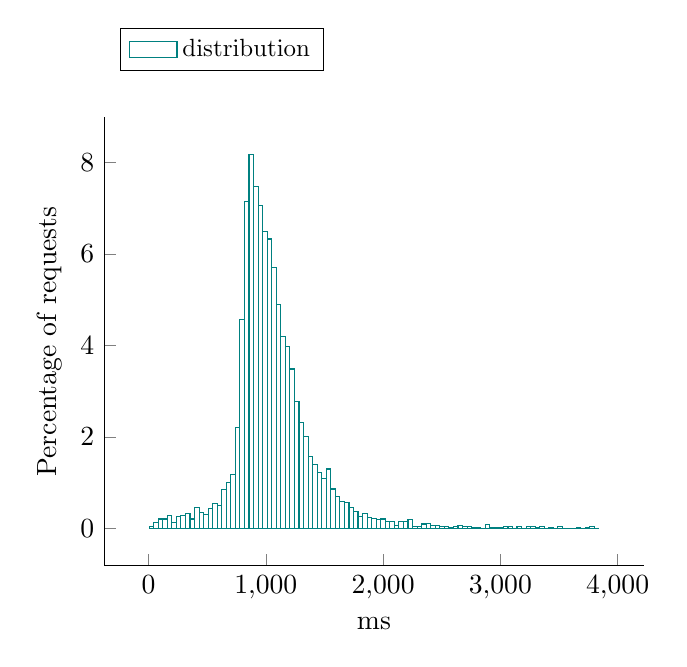
\begin{tikzpicture}
            \begin{axis}[ylabel = Percentage of requests, 
xlabel = ms, 
legend style = {nodes={scale=0.9, transform shape}, at={(0.03,1.2)}, anchor=north west, draw=black, fill=white, align=left, legend columns=3},
area style, mark size = 0pt,
 cycle list name = exotic,
  axis lines* = left]
		\addplot +[ybar interval] coordinates {
			 (5, 0.046875)
			 (43.73, 0.125)
			 (82.46, 0.203125)
			 (121.19, 0.203125)
			 (159.92, 0.28125)
			 (198.65, 0.125)
			 (237.38, 0.265625)
			 (276.11, 0.28125)
			 (314.84, 0.328125)
			 (353.57, 0.203125)
			 (392.3, 0.453125)
			 (431.03, 0.34375)
			 (469.76, 0.296875)
			 (508.49, 0.4375)
			 (547.22, 0.546875)
			 (585.95, 0.5)
			 (624.68, 0.84375)
			 (663.41, 1)
			 (702.14, 1.17188)
			 (740.87, 2.20312)
			 (779.6, 4.5625)
			 (818.33, 7.14062)
			 (857.06, 8.17188)
			 (895.79, 7.48438)
			 (934.52, 7.0625)
			 (973.25, 6.5)
			 (1011.98, 6.32812)
			 (1050.71, 5.70312)
			 (1089.44, 4.89062)
			 (1128.17, 4.1875)
			 (1166.9, 3.96875)
			 (1205.63, 3.48438)
			 (1244.36, 2.76562)
			 (1283.09, 2.3125)
			 (1321.82, 2.01562)
			 (1360.55, 1.57812)
			 (1399.28, 1.39062)
			 (1438.01, 1.21875)
			 (1476.74, 1.09375)
			 (1515.47, 1.29688)
			 (1554.2, 0.859375)
			 (1592.93, 0.6875)
			 (1631.66, 0.578125)
			 (1670.39, 0.5625)
			 (1709.12, 0.453125)
			 (1747.85, 0.375)
			 (1786.58, 0.25)
			 (1825.31, 0.328125)
			 (1864.04, 0.234375)
			 (1902.77, 0.21875)
			 (1941.5, 0.1875)
			 (1980.23, 0.203125)
			 (2018.96, 0.15625)
			 (2057.69, 0.140625)
			 (2096.42, 0.0625)
			 (2135.15, 0.140625)
			 (2173.88, 0.140625)
			 (2212.61, 0.1875)
			 (2251.34, 0.046875)
			 (2290.07, 0.03125)
			 (2328.8, 0.09375)
			 (2367.53, 0.109375)
			 (2406.26, 0.0625)
			 (2444.99, 0.0625)
			 (2483.72, 0.03125)
			 (2522.45, 0.03125)
			 (2561.18, 0.015625)
			 (2599.91, 0.046875)
			 (2638.64, 0.0625)
			 (2677.37, 0.046875)
			 (2716.1, 0.046875)
			 (2754.83, 0.015625)
			 (2793.56, 0.015625)
			 (2832.29, 0)
			 (2871.02, 0.078125)
			 (2909.75, 0.015625)
			 (2948.48, 0.015625)
			 (2987.21, 0.015625)
			 (3025.94, 0.03125)
			 (3064.67, 0.03125)
			 (3103.4, 0)
			 (3142.13, 0.046875)
			 (3180.86, 0)
			 (3219.59, 0.046875)
			 (3258.32, 0.03125)
			 (3297.05, 0.015625)
			 (3335.78, 0.03125)
			 (3374.51, 0)
			 (3413.24, 0.015625)
			 (3451.97, 0)
			 (3490.7, 0.03125)
			 (3529.43, 0)
			 (3568.16, 0)
			 (3606.89, 0)
			 (3645.62, 0.015625)
			 (3684.35, 0)
			 (3723.08, 0.015625)
			 (3761.81, 0.03125)
			 (3800.54, 0)
			 (3839.27, 0.015625)
		};
\addlegendentry{distribution};
           \end{axis}
      \end{tikzpicture}
  \end{adjustbox}
  \caption{Response time distribution - req = ReadTimeline-1}
\end{figure}
\end{minipage}\hfill\begin{minipage}{0.18\linewidth}
\begin{table}[h]
\begin{tabular}{|cc|}
\hline
\textbf{} & \textbf{ms}\\ \hline
 \Xhline{0.005\arrayrulewidth}
min & 5\\
 \Xhline{0.005\arrayrulewidth}
max & 3878\\
 \Xhline{0.005\arrayrulewidth}
mean & 1066\\
 \Xhline{0.005\arrayrulewidth}
std & 358\\
\hline
\hline
 \Xhline{0.005\arrayrulewidth}
25th & 876\\
 \Xhline{0.005\arrayrulewidth}
50th & 1007\\
 \Xhline{0.005\arrayrulewidth}
75th & 1197\\
 \Xhline{0.005\arrayrulewidth}
80th & 1254\\
 \Xhline{0.005\arrayrulewidth}
85th & 1333\\
 \Xhline{0.005\arrayrulewidth}
90th & 1455\\
 \Xhline{0.005\arrayrulewidth}
95th & 1663\\
 \Xhline{0.005\arrayrulewidth}
99th & 2394\\
\hline
\end{tabular}
\caption{Response time}
\end{table}
\end{minipage}\hfill